\subsection{Mittellinie \dcfirstauthorshort}
\label{ssec:fahrspurerkennung_punkt:verifikation:mittellinie}
Die Prozedur der Verifizierung verläuft nach einem vergleichbaren Prinzip wie der in Abschnitt~\ref{ssec:fahrspurerkennung:riverflow:randlinie} beschriebene Riverflow-Algorithmus. Dabei wird davon ausgegangen, dass sich das Fahrzeug größtenteils in der Fahrspur befindet, sodass mindestens ein Mittellinienstrich unweit vor dem Auto positioniert ist. Initial wird ein Suchfenster erstellt, welches in der Höhe den reichlichen Abstand zwischen den Mittelpunkten zweier benachbarter Mittelstreifen annimmt. Das erste sich in diesem Bereich aufhaltende Objekt wird dann als verifiziert angesehen, wenn seine Orientierung nicht übermäßig von der des Fahrzeugs abweicht. Ausgehend von diesem Punkt \glqq hangelt\grqq{} sich der Verifikations-Algorithmus von Strich zu Strich, indem er eine neue \gls{acr:roi} (ein neues Suchfenster) aufstellt. Da zu jedem (verifizierten) Punkt seine Orientierung bekannt ist, wird der nächste Mittellinienpunkt in dieser Richtung im ebenfalls bekannten Abstand zwischen zwei Punkten vermutet und dort der Mittelpunkt des neuen Suchfensters definiert. Dieses Schema wiederholt sich, bis entweder der Bildrand erreicht ist, keine Punkte im Suchfenster liegen, oder sich die Orientierung von einem zum nächsten Strich zu stark geändert hat.

Das gleiche Vorgehen wird zudem wahlweise vom ersten Punkt hinter dem Fahrzeug ausgehend wiederholt, sodass auch schon passierte Mittellinienpunkte, welche z.B. bei einem zukünftig implementierten Überholvorgang benötigt werden könnten, verifiziert sind.

\begin{figure}[htbp]
	\centering
	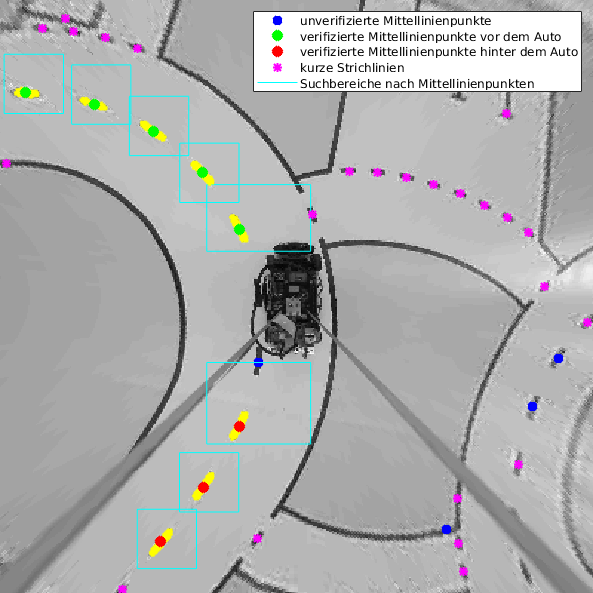
\includegraphics[width=0.9\textwidth]{fahrspurerkennung_riverflow_regionprops.png}
	\caption{Detektion von Punktgruppen mit bestimmten Eigenschaften mithilfe der \emph{regionprops}-Funktion}
	\label{fig:riverflow:mittellinie:regionprops}
\end{figure}

In Abb.~\ref{fig:riverflow:mittellinie:regionprops} sehen wir das Resultat der Mittellinien-/Stricherkennung. Im gleichen Zug wird die \emph{regionprops}-Funktion auch zur Randstricherkennung bei Kreuzungen genutzt. Die Verarbeitung dieser Informationen kommt im Riverflow-Algorithmus während des Sonderfalls einer unterbrochenen Randlinie zum Einsatz, welcher im Abschnitt~\ref{sssec:fahrspurerkennung:riverflow:randlinie:gestrichelt} näher beschrieben ist.